\documentclass[a4paper,12pt]{report}

\usepackage{alltt, fancyvrb, url}
\usepackage{graphicx}
\usepackage[utf8]{inputenc}
\usepackage{hyperref}
\usepackage{setspace}

% Questo commentalo se vuoi scrivere in inglese.
\usepackage[italian]{babel}

\usepackage[italian]{cleveref}

\title{Relazione\break``Farming Simulator''}

\author{Linda Fabbri, \\ Federico Raffoni,\\ Simone Rega,\\ Giacomo Montali}
\date{20 Aprile 2021}


\begin{document}

\maketitle

\tableofcontents

\chapter{Analisi}


\section{Requisiti}


Il gruppo si pone come obiettivo quello di realizzare "Farming Simulator", un software a scopo ludico basato sul videogioco "Hay Day" \footnote{\url{https://supercell.com/en/games/hayday/}} sviluppato da Supercell.
Il progetto mira alla realizzazione di un ambiente agricolo in 2D, in cui il giocatore interagisce con le colture e gestisce le proprie finanze.
Lo scopo del gioco è arrivare all'apice della ricchezza, sbloccando tutti gli appezzamenti di terra e coltivando la maggior varietà di semi possibili.


\subsubsection{Requisiti funzionali}
\begin{itemize}
	\item Questa applicazione deve permettere al giocatore di muoversi all'interno della mappa di gioco evitando di salire su zone di mappa non calpestabili.
	\item Il personaggio ha la possibilità di coltivare piantagioni di grano, patate, pomodori, carote, alberi di ciliege e altri frutti.
	\item Nella mappa deve comparire una zona per l'allevamento degli animali, grazie ai quali si possono raccogliere latte, uova e altri derivati.
	\item Farming Simulator mette a disposizione un negozio in cui è possibile vedere il proprio inventario, vendere i prodotti agricoli raccolti in cambio di monete virtuali e comprare nuovi semi da coltivare.
	\item Per aumentare la difficoltà di gioco vengono messi a disposizione appezzamenti di terreno coltivabili inizialmente bloccati, che si possono sbloccare tramite l'utilizzo delle monete virtuali.
\end{itemize}


\subsubsection{Requisiti non funzionali}
\begin{itemize}
	\item Farming Simulator deve poter essere eseguito su dispositivi con schermi dotati di risoluzioni differenti.
	\item Il programma deve poter essere eseguito sia su Windows sia su sistemi operativi Unix
\end{itemize}

\hfill\break
\section{Analisi e modello del dominio}

In Farming Simulator il soggetto principale è il personaggio virtuale, il quale si muove all'interno di una mappa, composta da diversi tipologie di blocchi. 

All'interno della mappa possiamo trovare blocchi coltivabili (Field Block), blocchi non calpestabili dal personaggio (Wall), blocchi estetici(Water), il quale unico compito è quello di abbellire la mappa, blocchi che compongono la stalla in cui possono muoversi gli animali(Stall), ed infine blocchi "locked"(Unlockable Block), ovvero che inizialmente sono bloccati e possono essere sbloccati durante la partita in cambio di monete virtuali.

Il personaggio (Player), grazie all'inventario (Inventory), è in grado di mantenere risorse al suo interno. Tra le risorse collezionabili possiamo trovare: il cibo (Food) ottenuto dalla raccolta di coltivazioni o di animali oppure i semi (Seed).
Questi ultimi possono essere comprati nel negozio (Shop) del videogioco, dentro il quale è anche possibile vendere il cibo che si è raccolto.

Il personaggio può interaggire con blocchi e animali (Animals), in particolare può piantare e raccogliere i semi all'interno dei blocchi coltivabili (FieldBlock), sbloccare i blocchi non ancora accessibili (UnlockableBlock) e raccogliere i prodotti animali.

\begin{figure}[!htb]
\centerline{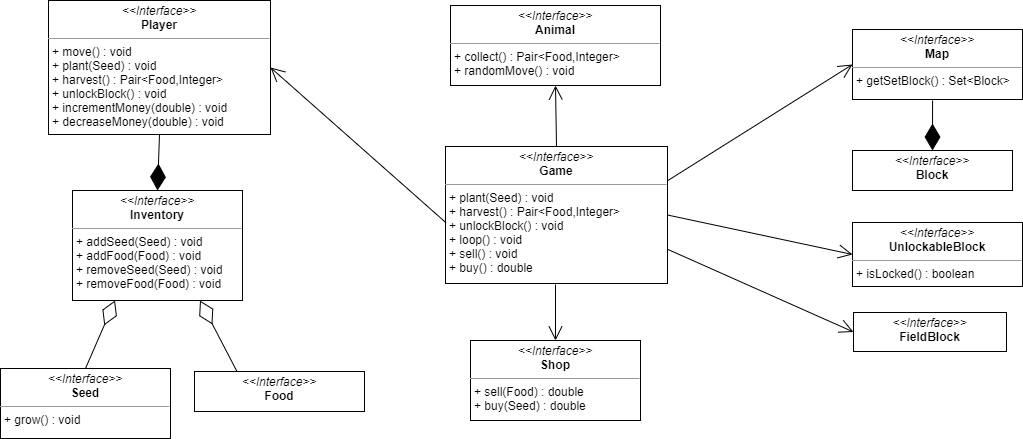
\includegraphics[width=\textwidth]{img/UML_1-1.png}}
\caption{Schema UML dell'analisi del problema, con rappresentate le entità principali ed i rapporti fra loro}
\label{img:analysis}
\end{figure}

\chapter{Design}

\section{Architettura}

L’architettura di Farming Simulator è basata su un pattern MVC. In particolare è stata sviluppata l’interfaccia Game che funge da Controller e si posiziona tra View e Model e gestisce eventuali interazioni tra componenti. All’arrivo di un input, game, si occupa di ordinare al Model il cambio di stato.

\hfill\break
Gli input da tastiera provenienti dall’utente passano attraverso la classe KeyNotifier, la quale si occupa di informare il game dell’avvenuto input. 

\hfill\break
La parte di View è formata da diversi GameDrawer, i quali si occupano di interrogare il game e mostrare a video il gioco.

Quando viene catturato un input da tastiera, il GameDrawer avvisa il keyNotifier dell’avvenuta pressione, così facendo il KeyNotifier è un observable per GameDrawer. In questo modo il GameDrawer non si deve occupare della gestione degli input, spostando il carico di lavoro al KeyNotifier; questa astrazione ci permette di non dipendere dall'implementazione e poter cambiare il binding\footnote[1]{Binding = associazione di un tasto ad un determinato movimento e/o interazione visiva in gioco (ad esempio [WASD] per spostarsi nella mappa)} o addirittura dispositivo di input (ad esempio un Joystick). 

\hfill\break
In \Cref{img:MVC} è esemplificato il diagramma UML che descrive l'architettura MVC del progetto, mostrando le classi principali.

\hfill\break
\begin{figure}[!htb]
\centerline{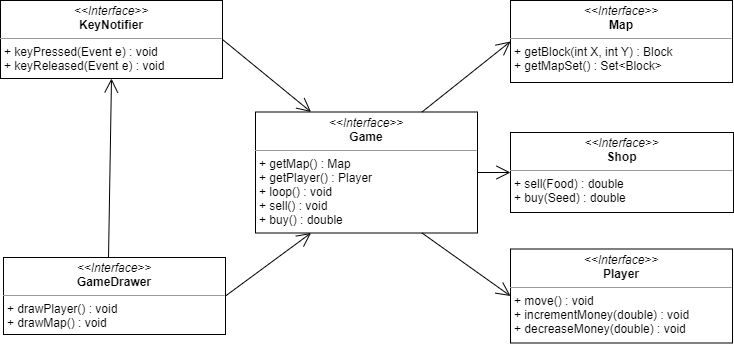
\includegraphics[scale=.65]{img/UML_2-1.png}}

\caption{Schema UML architetturale di Farming Simulator, MVC.}
\label{img:MVC}
\end{figure}





\section{Design dettagliato}

In questa sezione vengono mostrati alcuni elementi di design con maggior dettaglio.
Ogni membro del gruppo presenta gli elementi di design più significativi da lui prodotti, al fine di realizzare l’applicazione, predisponendola a future espansioni.



\subsection{Simone Rega}
Io nel progetto mi sono occupato della parte riguardante l’aggiornamento dinamico della GUI nella sezione dello Shop, in particolare mi preoccupo di aggiornare il JPanel dello shop e la visualizzazione dell’inventario ogni qualvolta che si interagisce con i JButton di compra/vendita, la JComboBox e il JSpinner per comprare semi. 

Ho ritenuto utile usare un pattern Observer in modo che alla ricevuta notifica di un osservatore, quindi un Evento sui componenti grafici descritti prima, gli altri osservatori vengono notificati per poi essere aggiornati.

\hfill\break
È stato deciso insieme a\textit{ Federico Raffoni} di creare le interfacce \textbf{Observer} e \textbf{Observable} di tipo generico, in modo da poter implementare le classi in più possibili situazioni eterogenee.
Il ruolo di Observable è ricoperto dalla classe ObservableShopGUI mentre il ruolo di Observer è ricoperto da ObserverShop (classe innestata all’interno di ShopDrawer.java). 

\hfill\break
In \Cref{img:SimoneRega_Observer} è esemplificato il diagramma UML che descrive l'architettura del pattern Observer usato da Simone Rega, mostrando le classi principali.
\hfill\break

\begin{figure}[!htb]
	\centerline{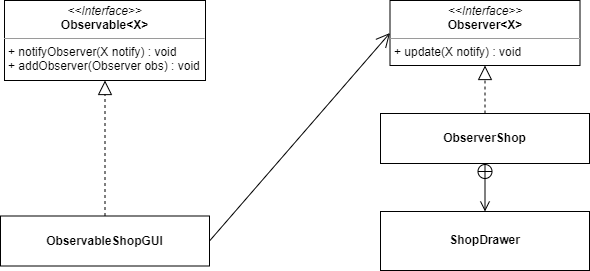
\includegraphics[scale=0.8]{img/UML_ObserverSimo.png}}
	
	\caption{Schema UML architetturale del pattern Observer (Simone Rega).}
	\label{img:SimoneRega_Observer}
\end{figure}

\subsection{Federico Raffoni}
In questa sezione ci occuperemo principalmente del caricamento delle risorse grafiche e non solo. In particolare è stata creata la classe Resources la quale si occupa di caricare e distribuire tutte le risorse. 

È stato usato il pattern SINGLETON per rendere unico nell’applicazione l’accesso alla classe Resources. In questo modo si evita che diversi GameDrawer carichino più volte le risorse sprecando memoria.

 Le risorse verranno caricate solo alla prima chiamata, mentre le chiamate successive riceveranno una copia statica della classe risparmiando tempo e risorse.
 
 In \Cref{img:FedericoRaffoni_Singleton} è esemplificato il diagramma UML che descrive l'architettura singleton, mostrando le classi principali.
\hfill\break

\begin{figure}[!htb]
	\centering{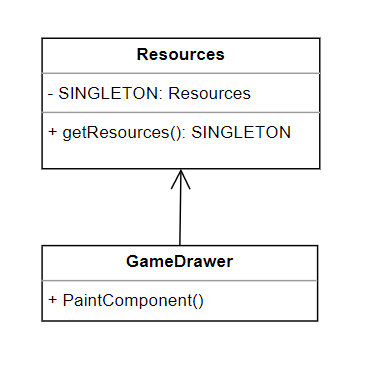
\includegraphics[scale=.6]{img/UML_SingletonRaffo.png}}
	\caption{Schema UML architetturale del pattern Singleton (Federico Raffoni).}
	\label{img:FedericoRaffoni_Singleton}
\end{figure}

Per quanto riguarda il caricamento di una partita salvata, è stato utilizzato il pattern Observer per consentire all’Engine di rimanere in attesa mentre la classe GamePreloader si occupa di chiedere alll’utente se continuare una partita salvata oppure iniziare una partita da zero.

In particolare Engine è Observer, mentre la classe GamePreloader è Observable.  Sono state realizzate inoltre le interfacce Observer e Observable generiche, in modo da poter essere riutilizzate anche in altri campi.

 In \Cref{img:FedericoRaffoni_Observer} è esemplificato il diagramma UML che descrive l'architettura Observer, mostrando le classi principali.

\hfill\break
\begin{figure}[!htb]
	\centering{}
	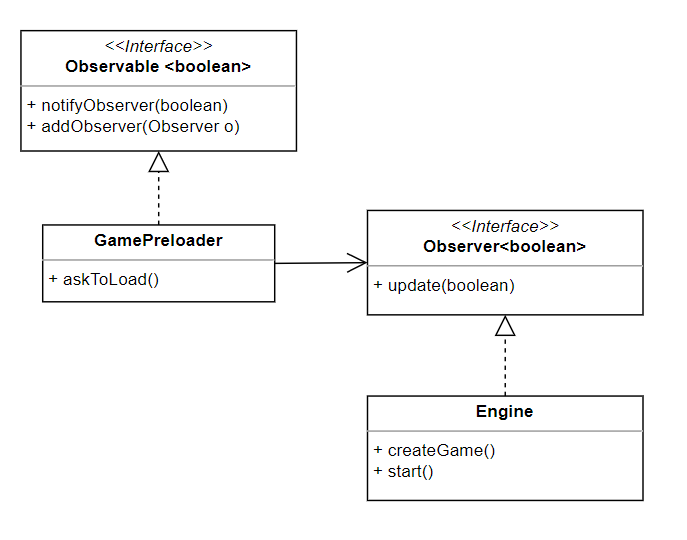
\includegraphics[width=\textwidth]{img/UML_ObserverRaffo.png}
	\caption{Schema UML architetturale del pattern Observer (Federico Raffoni).}
	\label{img:FedericoRaffoni_Observer}
\end{figure}

\subsection{Linda Fabbri}
La parte di progetto riguardo al design di cui mi sono occupata personalmente è quella riguardante i blocchi. 

Questa parte è composta da una classe enum (BlockType) per la classificazione delle tipologie dei vari blocchi, in base alla tipologia ho avuto la necessità di implementare metodi diversi, dunque ho creato tre interfacce: \textbf{Block} per tutti i generici blocchi, \textbf{FieldBlock} (estensione di Block) a cui ho aggiunto i metodi per i blocchi coltivabili (FIELD in BlockType), \textbf{UnlockableBlock}(estensione di FieldBlock) a cui ho aggiunto i metodi per i blocchi coltivabili bloccati (LOCKED in BlockType).

L’implementazione di queste interfacce si trova in FactoryBlock come classi innestate. Inoltre, per ogni tipologia di blocco si ha un differente costruttore al fine di determinare i vari campi. 

Ho scelto l’utilizzo del pattern \textit{“Factory method”} allo scopo di creare e ritornare blocchi in base al loro tipo mediante l’uso di costruttori differenti, delegando la responsabilità della scelta della creazione di ogni oggetto solo alla classe che implementa tale pattern.

In \Cref{img:LindaFabbri_Factory} è esemplificato il diagramma UML che descrive l'architettura Factory Method, mostrando le classi principali.

\hfill\break
\begin{figure}[!htb]
	\centerline{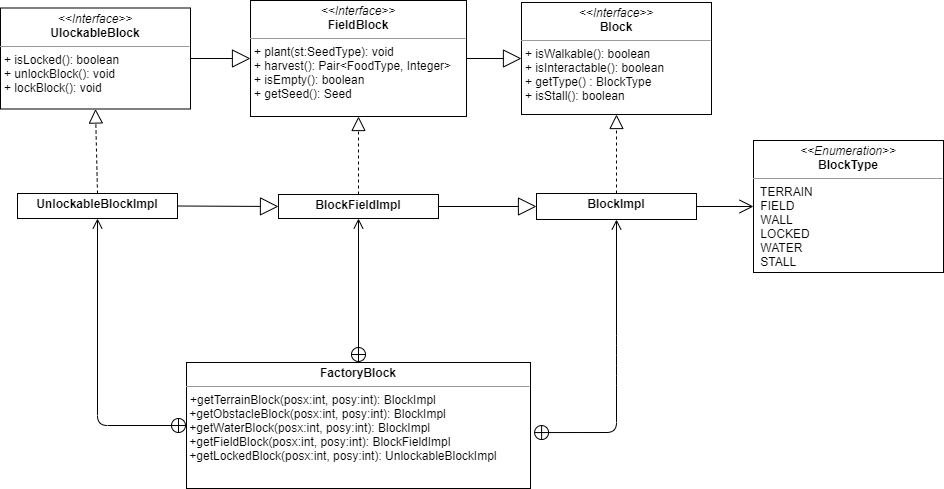
\includegraphics[scale=.5]{img/UML_FactoryLinda.png}}	
	\caption{Schema UML architetturale del pattern Factory Method (Linda Fabbri).}
	\label{img:LindaFabbri_Factory}
\end{figure}

\subsection{Giacomo Montali}

I principali punti dei quali mi sono occupato in questo progetto sono le varie entità presenti in essa, cioè il Player e i vari animali. 

In particolare per questi ultimi ho utilizzato il pattern \textit{“Simple Factory”}  nella classe \textbf{FactoryAnimal}, con l’obiettivo di delegare la creazione degli animali a quest’ultima, separandola così dalla classe \textbf{AnimalImpl} per  rendere più facile l'aggiunta di eventuali nuovi classi che implementano l'interfaccia Animal. 

La suddivisione degli animali è stata effetuata grazie ad un Enum.

\begin{figure}[!htb]
	\centering{}
	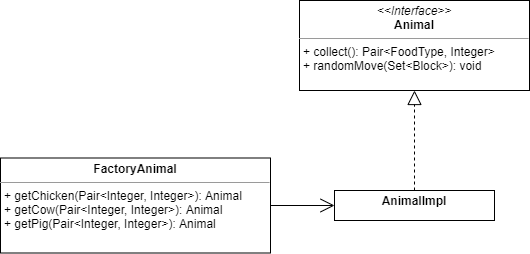
\includegraphics[width=\textwidth]{img/UML_FactoryMonta.png}
	\caption{Schema UML architetturale del pattern Simple Factory (Giacomo Montali).}
	\label{img:GiacomoMontali_Factory}
\end{figure}

In \Cref{img:GiacomoMontali_Factory} è esemplificato il diagramma UML che descrive l'architettura del Pattern Simple Factory, mostrando le classi principali.

Inoltre ho creato la classe abstract \textbf{Entity} per renderla classe padre delle classi \textbf{PlayerImpl} e \textbf{AnimalImpl}, per evitare il riutilizzo di codice derivato dai metodi in comune come tutti i metodi che riguardano il movimento e la posizione sulla mappa.

In \Cref{img:GiacomoMontali_Abstract} è esemplificato il diagramma UML che descrive l'architettura delle classe Abstract Entity, mostrando le classi principali.

\hfill\break
\begin{figure}[!htb]
	\centering{}
	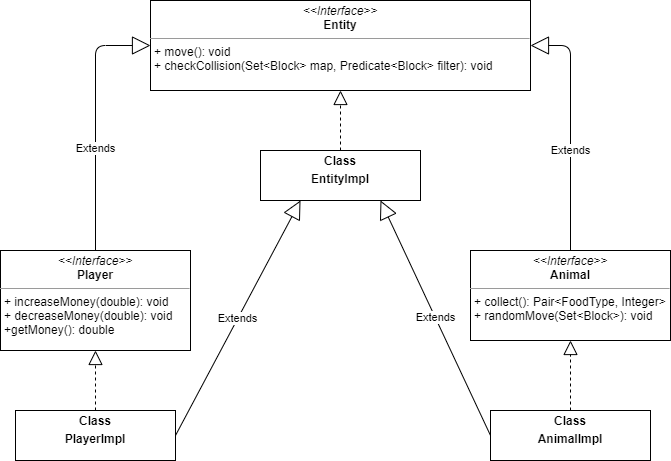
\includegraphics[width=\textwidth]{img/UML_AbstractMonta.png}
	\caption{Schema UML architetturale della classe Entity (Giacomo Montali).}
	\label{img:GiacomoMontali_Abstract}
\end{figure}

\chapter{Sviluppo}
\section{Testing automatizzato}


In questo progetto abbiamo deciso di testare prevalentemente la parte di Model poiché riteniamo sia la più propensa ad avere bug; non sono però mancati test riguardanti la View e salvataggio del gioco.
Per svolgere test completamente automatizzati sul progetto è stato usato JUnit5.


{\setstretch{0.6}
Le classi che sono state testate sono:
\begin{itemize}
	\item \textbf{testPlayerMovement:} con questo test muovo il personaggio simulando la pressione dei tasti  
	\item \textbf{testPlayerCollision:} con questo test controllo che non avvenga il movimento su blocchi o in direzioni in cui mi è permesso
	\item \textbf{testPlayerPlant:} con questo test simulo l'interazione del personaggio con un blocco di tipo FieldBlock, piantando un seme e poi controllando che quel blocco non sia vuoto
	\item \textbf{testUnlockBlock:} con questo test simulo l'interazione con un blocco di tipo UnlockableBlock
	\item \textbf{testUnlockBlockWithoutMoney:} con questo test simulo l'interazione con un blocco di tipo UnlockableBlock senza soldi
	\item \textbf{testPlayerAnimalInteraction:} con questo test mi sposto nella zona "Stalla" della mappa e aspetto che un Animal qualunque sia pronto per poi poter raccogliere il suo \textit{Food} simulando l'interazione tra \textit{Player} e \textit{Animal}
	\item \textbf{testBuy:} con questo test provo a comprare un \textit{Seed} dallo \textit{Shop}, controllando poi che sia effettivamente presente nell'\textit{Inventory}
	\item \textbf{testBuyWithoutMoney:} questo test è simile al precedente, ma ho zero money, verificando che non avvenga l'acquisto
	\item \textbf{testSell:} in questo test simulo una normale interazione con un FieldBlock, ricavandone poi il raccolto che proverò a vendere, verificandone l'esistenza nell'inventario e l'ottenimento dei soldi ricavati dalla vendita
	\item \textbf{testSaver:} con questo test simulo il salvataggio del gioco su file con relativa apertura da esso in una nuova esecuzione del gioco, verificando che i nuovi e vecchi \textit{Game} e \textit{Player} siano gli stessi e abbiano le stesse caratteristiche
	\item \textbf{testSaverPlayer:} questo test è simile al precedente, differisce semplicemente per il fatto che il Player viene mosso nella nuova istanza di gioco, così da far risultare falso il fatto che l'istanza salvata e l'istanza nuova creata siano uguali	
\end{itemize}
}



\section{Metodologia di lavoro}

\textbf{• Metodologia riguardante il progetto in generale}\hfill\break
Lo sviluppo del progetto è stato preceduto da una fase preliminare di analisi e progettazione, durante la quale abbiamo lavorato tutti insieme per definire prima le basi dell'applicazione, poi successivamente specificare i vari dettagli implementativi tramite UML sulla piattaforma Miro.

In queste fasi la collaborazione e il confronto sono state molto intense.

La suddivisioni delle parti di Farming Simulator  è avvenuta in modo abbastanza equo assegnando a ciascuno una parte significativa e importante del progetto, anche in base alle nostre preferenze. 

\hfill\break
\textbf{• Distributed Version Control System}\hfill\break
Come DVCS è stato usato Git, creando un repository su GitHub. Abbiamo lavorato sullo scheletro del progetto su un unico branch main, per poi creare diversi branch per implementare e/o mettere a punto la realizzazione di feature nuove o più sostanziose.

\subsection{Federico Raffoni}
Sviluppo del motore grafico, in particolare l’Engine e la classe WindowManager, e le varie interazioni tra questi due elementi. Ideazione e creazione della classe abstract GameDrawer che ha portato alla realizzazione delle varie scene di gioco.  Sviluppo della classe KeyNotifier che permette l’interazione tra la view e il controller (Game).

 Implementazione della classe Resources. 
 
 Ho inoltre sviluppato la classe che permette il salvataggio e il caricamento della partita (GameSaver) .

\hfill\break
Ho inoltre contribuito all'implementazione della classe Game  e  allo sviluppo della parte grafica nella classe MainScreenDrawer 

\hfill\break
Classi sviluppate singolarmente:
{\setstretch{0.6}
\begin{itemize}
	\item KeyNotifier
	\item Engine
	\item GameSaver
	\item GameDrawer
	\item GamePreloader
	\item Resources
	\item WindowManager
	\item MusicPlayer
\end{itemize}
}

\subsection{Linda Fabbri}

Si è occupata principalmente della parte riguardante la logica di gioco legata alle interazioni fra le entità e la parte che si occupa della creazione dei blocchi che compongono la mappa di gioco, in particolare le classi Interaction, InteractionImpl nel package engine e tutte le classi del package block. 

Legato alle interazioni ha implementato i metodi riguardanti la compravendita di prodotti che si trovano nella classe ShopImpl, in particolare i metodi sellAll e buy. 

In collaborazione con Simone Rega si è implementata la classe ShopDrawer per la parte che si occupa della grafica dei pannelli legati alla compravendita di semi e prodotti. 

Ha collaborato all’implementazione della classe Game, in particolare per chiamare i metodi implementati in InteractionImpl. 

In collaborazione con Simone Rega e Federico Raffoni ha eseguito il refactoring per correggere errori evidenziati dal checkstyle.

\hfill\break
\textbf{•Problemi}\hfill\break
In fase di progettazione nella classe Inventory si era pensato di creare solo i metodi gotFoods e gotSeeds, per verificare l’esistenza di un certo numero di Food o Seed nell’inventario, tuttavia per i metodi delle classi che sono state citate precedentemente, si è trovata la necessità di un metodo che ritornasse la mappa di tutte le tipologie di Food e Seed.

\subsection{Simone Rega}
Sviluppo delle classi all'interno del package Item che riguardano principalmente la realizzazione degli elementi Seed e Food del gioco.

Sviluppo della parte di grafica riguardante lo shop (ShopDrawer); le informazioni del gioco (InfoDrawer e implementazione di vari JPanelHUD nel MainScreenDrawer).

Ideazione e creazione delle classi nel package gameShop riguardante la logica base dello Shop

Ideazione e sviluppo della classe test in JUnit5 a cui hanno dato una mano allo sviluppo Linda Fabbri e Federico Raffoni.

\hfill\break
Classi sviluppate singolarmente:
{\setstretch{0.6}
\begin{itemize}
	\item FoodType
	\item SeedType
	\item Seed
	\item SeedImpl
	\item ItemConstants
	\item UnlockableBlock
	\item InfoDrawer
	\item QuitDrawer
	\item JPanelINFO
	\item JPanelHUD
	\item ObservableShopGUI
\end{itemize}
}
\hfill\break

Classi sviluppate insieme ad altre persone
{\setstretch{0.6}
\begin{itemize}
	\item MainScreenDrawer : implementazione di generateHUD per generare la barra di gioco superiore
	\item ShopDrawer : quasi tutta la parte grafica
	\item FarmingSimulatorTestClass 
	\item Observer
	\item Observable
	\item Shop
	\item ShopImpl
\end{itemize}
}

\subsection{Giacomo Montali}
Sviluppo del package entity, che riguarda principalmente Player, Animal e le relative classi ad esse connesse.

Sviluppo della mappa di gioco dentro la quale interagiranno le entità. Caricamento della mappa di gioco da file.

\section{Note di sviluppo}

\subsection{Federico Raffoni}

\begin{itemize}
	\item \textbf{Lambda:} ho usato le lambda all’interno del metodo loop della classe GameImpl per muovere tutte le entità e per impostare i blocchi camminabili dal player
	\item\textbf{Reflection:} All’interno della classe GameSaver
\end{itemize}

Ho utilizzato la libreria Gson per serializzare e deserializzare i componenti di gioco per permettere il salvataggio e il caricamento della partita.
Nell’implementazione della classe GameSaver è stato necessario sviluppare un serializzatore di interfacce il quale è stato scritto prendendo spunto da questo thread (source: https://stackoverflow.com/questions/62358189/gson-stackoverflowerror-during-serialization)

Per la creazione della classe MusicPlayer, non essendo pratico delle funzioni di libreria di javax.sound, ho fatto riferimento a snippet presenti sul web


\subsection{Simone Rega}
Per quanto riguarda le Feature Avanzate del linguaggio: 
\begin{itemize}
	\item \textbf{Lambda :} utilizzate nella classe FarmingSimulatorTestClass per i test sul Player e sui Blocchi	
	\item \textbf{IntStream: }utilizzate nella classe FarmingSimulatorTestClass .
\end{itemize}

\hfill\break
Per quanto riguarda le librerie utilizzate
\begin{itemize}
	\item \textbf{Java AWT }
	\item \textbf{Java Swing}
\end{itemize}
So che queste due librerie sono state introdotte a lezione spiegandone i principali elementi di maggior rilevanza ma ci tengo comunque a precisare lo studio e l'approfondimento per poter realizzare elementi di grafica più complessi o che purtroppo non abbiamo avuto modo di trattate a lezione .
 
\subsection{Linda Fabbri}

\begin{itemize}
	\item \textbf{Optional: } nei blocchi per il loro contenuto
	\item \
\end{itemize}


\subsection{Giacomo Montali}

\chapter{Commenti finali}

In quest'ultimo capitolo si tirano le somme del lavoro svolto e si delineano eventuali sviluppi
futuri.

\textit{Nessuna delle informazioni incluse in questo capitolo verrà utilizzata per formulare la valutazione finale}, a meno che non sia assente o manchino delle sezioni obbligatorie.
%
Al fine di evitare pregiudizi involontari, l'intero capitolo verrà letto dai docenti solo dopo aver formulato la valutazione.

\section{Autovalutazione e lavori futuri}

\subsection{Simone Rega}
Sin dall'inizio sono stato partecipe e disponibile per la progettazione e l'analisi del progetto. 

Purtroppo non ho potuto lavorare troppo sulla logica di gioco (ho semplicemente svolto la parte riguardante la logica che può avere un seme quando piantato)

Sono abbastanza contento del risultato finale riguardante il lavoro da me svolto e della modesta qualità del mio codice, che è stata equilibrata e trasparente, permettendone un corretto e utile uso.

Devo dire che sono leggermente dispiaciuto perché avrei voluto essere più partecipe o comunque dedicarmi di più allo sviluppo del programma. Avrei potuto migliorare l'ottimizzazione del mio codice e le sue funzionalità, o magari osare di più con elementi di programmazioni più avanzati introducendo più Lambda e Stream ad esempio. 

Sono contento del Team con cui ho avuto modo di lavorare a questo progetto. La comunicazione è stata di fondamentale importanza.

\subsection{Federico Raffoni}
\subsection{Linda Fabbri}
\subsection{Giacomo Montali}

\section{Difficoltà incontrate e commenti per i docenti}

\subsection{Simone Rega}

buon corso, oop uni > iti
gradle spiegata meglio

Purtroppo il mio percorso di sviluppo non è stato lineare nel tempo; nonostante fosse stimolante per me avere per la prima volta un progetto di programmazione così bello e complesso da portare avanti, questo non è stato sempre possibile poiché non sempre sono riuscito a trovare il tempo per dedicarmi ad esso dopo le lezioni o lo studio. È effettivamente il primo progetto di sviluppo software da zero a cui ho partecipato e mi ha fatto crescere dal punto di vista organizzativo, rendendomi cosciente di ciò che mi aspetta una volta uscito dall'università.
\subsection{Federico Raffoni}
\subsection{Linda Fabbri}
\subsection{Giacomo Montali}
\appendix
\chapter{Guida utente}

Capitolo in cui si spiega come utilizzare il software. Nel caso in cui il suo uso sia del tutto
banale, tale capitolo può essere omesso.
%
A tal riguardo, si fa presente agli studenti che i docenti non hanno mai utilizzato il software
prima, per cui aspetti che sembrano del tutto banali a chi ha sviluppato l'applicazione possono non
esserlo per chi la usa per la prima volta.
%
Se, ad esempio, per cominciare una partita con un videogioco è necessario premere la barra
spaziatrice, o il tasto ``P'', è necessario che gli studenti lo segnalino.

\subsection*{Elementi positivi}

\begin{itemize}
 \item Si istruisce in modo semplice l'utente sull'uso dell'applicazione, eventualmente facendo uso di schermate e descrizioni.
\end{itemize}

\subsection*{Elementi negativi}
\begin{itemize}
 \item Si descrivono in modo eccessivamente minuzioso tutte le caratteristiche, anche minori, del software in oggetto.
 \item Manca una descrizione che consenta ad un utente qualunque di utilizzare almeno le funzionalità primarie dell'applicativo.
\end{itemize}

\chapter{Esercitazioni di laboratorio}

In questo capitolo ciascuno studente elenca gli esercizi di laboratorio che ha svolto
(se ne ha svolti),
elencando i permalink dei post sul forum dove è avvenuta la consegna.

\section*{Esempio}

\subsection{Paolino Paperino}

\begin{itemize}
 \item Laboratorio 04: \url{https://virtuale.unibo.it/mod/forum/discuss.php?d=12345#p123456}
 \item Laboratorio 06: \url{https://virtuale.unibo.it/mod/forum/discuss.php?d=22222#p222222}
 \item Laboratorio 09: \url{https://virtuale.unibo.it/mod/forum/discuss.php?d=99999#p999999}
\end{itemize}

\subsection{Paperon De Paperoni}

\begin{itemize}
 \item Laboratorio 04: \url{https://virtuale.unibo.it/mod/forum/discuss.php?d=12345#p123456}
 \item Laboratorio 05: \url{https://virtuale.unibo.it/mod/forum/discuss.php?d=22222#p222222}
 \item Laboratorio 06: \url{https://virtuale.unibo.it/mod/forum/discuss.php?d=99999#p999999}
 \item Laboratorio 07: \url{https://virtuale.unibo.it/mod/forum/discuss.php?d=22222#p222222}
 \item Laboratorio 08: \url{https://virtuale.unibo.it/mod/forum/discuss.php?d=99999#p999999}
 \item Laboratorio 09: \url{https://virtuale.unibo.it/mod/forum/discuss.php?d=22222#p222222}
 \item Laboratorio 10: \url{https://virtuale.unibo.it/mod/forum/discuss.php?d=99999#p999999}
 \item Laboratorio 11: \url{https://virtuale.unibo.it/mod/forum/discuss.php?d=22222#p222222}
\end{itemize}


\bibliographystyle{alpha}
\bibliography{13-template}

\end{document}
